%%%%%%%%%%%%%%%%%%%%%%%%%%%%%%%%%%%%%%%%%%%%%%%%%%%%%%%%
% Canonical : https://github.com/lduran2/ece3413_classical_control_systems/doc/lab0405.tex
% Lab report
% By        : Leomar Duran <https://github.com/lduran2>
% When      : 2022-03-29t00:05Q
% For       : ECE 3413
% Version   : 1.2.0
%%%%%%%%%%%%%%%%%%%%%%%%%%%%%%%%%%%%%%%%%%%%%%%%%%%%%%%%
\documentclass[11pt]{article}
\usepackage[utf8]{inputenc}

\usepackage{lib/ccsreport}

\begin{document}

\title{ECE 3413 Lab 04/05 Time Response of First- and\\* Second-Order Systems}
\author{Leomar Durán}
\date{28\(^{\text{th}}\) March 2022}

\maketitle

\section*{Revision History}

\begin{tabularx}\linewidth{@{}rlrX@{}}
    \toprule
        Revision \#
            & Author
            & Revision date
            & Comments
    \\*
    \midrule
        1.2.0
            & Leomar Durán
            & 2022-03-29t00:05Q
            & explaining model of \(G_1(\cdot;\cdot)\)
    \\*
        1.1.0
            & Leomar Durán
            & 2022-03-28t22:09Q
            & introduction
    \\*
        1.0.0
            & Leomar Durán
            & 2022-03-28t21:39Q
            & initial lab 04/05
    \\*
        0.0.0
            & Leomar Durán
            & 2022-01-31t00:00R
            & template complete
    \\*
    \bottomrule
\end{tabularx}

\section{Introduction}

The purpose of this lab is
to evaluate the effects of poles, zeros and the gain
on first-order and second-order control systems.

After this lab, students will be able
to determine the effects of poles, zeros, and gain
as well the imaginary and real parts of poles,
and the damping ratio
on overshoot, settling time, rise time, peak time
and the overall shape of the step response.

Additionally, students will be able to plot the transient responses of systems, which include
the impulse response, step response, ramp response, and parabola response. The MATLAB \mintinline{matlab}{linearSystemAnalyzer} is also introduced as a tool for analysis.

\section{Procedure}

\begin{adjustwidth}{0.5in}{0in}
    \subsection{Part I}
        In Part I, we will practice by first performing modifications to the parametric first-order system
        \[
            G_1\brao{s; a} := \frac{a}{s + a},
        \]
        and analyze the resulting effects with the \mintinline{matlab}{linearSystemAnalyzer}.

        We will analyze \(G_1\brao{s;a}\) for \(a \in \brac{1..4}\). These systems are modelled by the Simulink subsystem in Fig. \ref{fig:1st order pole}.

        \begin{figure}
            \centering
            \includegraphics[
                page=2,%
                trim=3.375in 2.125in 3.375in 2.0625in,%
                clip,
                width=0.75\linewidth%
            ]{lab0405/fig/time_response_slx1.pdf}
            \caption{Part I: Manipulating the pole in a First-Order System.}
            \label{fig:1st order pole}
        \end{figure}

        Effectively, this is manipulation of the pole of \(G_1\brao{s;a}\). The gain is also changed simultaneously to keep the steady state value at \(1\). The steady state value is specified by \(\lim_{s\to0} G(s)\).
    \subsection{Part II}
    \subsection{Part III}
\end{adjustwidth}

\section{Results}
\section{Discussion}

\newpage
\appendix
\title{Appendix}\label{doc:apx}
\maketitle

\section{Codes and Commands used in the lab}

\begin{enumerate}
    \item
        \mintinline{matlab}{conv}
        \tabto{1.5in}
        \(\Rightarrow\) convolve or multiply polynomials
\end{enumerate}

\end{document}
